\documentclass[journal,12pt,twocolumn]{IEEEtran}

\usepackage{setspace}
\usepackage{gensymb}

\singlespacing


\usepackage[cmex10]{amsmath}

\usepackage{amsthm}

\usepackage{mathrsfs}
\usepackage{txfonts}
\usepackage{stfloats}
\usepackage{bm}
\usepackage{cite}
\usepackage{cases}
\usepackage{subfig}

\usepackage{longtable}
\usepackage{multirow}

\usepackage{enumitem}
\usepackage{mathtools}
\usepackage{steinmetz}
\usepackage{tikz}
\usepackage{circuitikz}
\usepackage{verbatim}
\usepackage{tfrupee}
\usepackage[breaklinks=true]{hyperref}

\usepackage{tkz-euclide}

\usetikzlibrary{calc,math}
\usepackage{listings}
    \usepackage{color}                                            %%
    \usepackage{array}                                            %%
    \usepackage{longtable}                                        %%
    \usepackage{calc}                                             %%
    \usepackage{multirow}                                         %%
    \usepackage{hhline}                                           %%
    \usepackage{ifthen}                                           %%
    \usepackage{lscape}     
\usepackage{multicol}
\usepackage{chngcntr}

\DeclareMathOperator*{\Res}{Res}

\renewcommand\thesection{\arabic{section}}
\renewcommand\thesubsection{\thesection.\arabic{subsection}}
\renewcommand\thesubsubsection{\thesubsection.\arabic{subsubsection}}

\renewcommand\thesectiondis{\arabic{section}}
\renewcommand\thesubsectiondis{\thesectiondis.\arabic{subsection}}
\renewcommand\thesubsubsectiondis{\thesubsectiondis.\arabic{subsubsection}}


\hyphenation{op-tical net-works semi-conduc-tor}
\def\inputGnumericTable{}                                 %%

\lstset{
%language=C,
frame=single, 
breaklines=true,
columns=fullflexible
}
\begin{document}


\newtheorem{theorem}{Theorem}[section]
\newtheorem{problem}{Problem}
\newtheorem{proposition}{Proposition}[section]
\newtheorem{lemma}{Lemma}[section]
\newtheorem{corollary}[theorem]{Corollary}
\newtheorem{example}{Example}[section]
\newtheorem{definition}[problem]{Definition}

\newcommand{\BEQA}{\begin{eqnarray}}
\newcommand{\EEQA}{\end{eqnarray}}
\newcommand{\define}{\stackrel{\triangle}{=}}
\bibliographystyle{IEEEtran}

\providecommand{\mbf}{\mathbf}
\providecommand{\pr}[1]{\ensuremath{\Pr\left(#1\right)}}
\providecommand{\qfunc}[1]{\ensuremath{Q\left(#1\right)}}
\providecommand{\sbrak}[1]{\ensuremath{{}\left[#1\right]}}
\providecommand{\lsbrak}[1]{\ensuremath{{}\left[#1\right.}}
\providecommand{\rsbrak}[1]{\ensuremath{{}\left.#1\right]}}
\providecommand{\brak}[1]{\ensuremath{\left(#1\right)}}
\providecommand{\lbrak}[1]{\ensuremath{\left(#1\right.}}
\providecommand{\rbrak}[1]{\ensuremath{\left.#1\right)}}
\providecommand{\cbrak}[1]{\ensuremath{\left\{#1\right\}}}
\providecommand{\lcbrak}[1]{\ensuremath{\left\{#1\right.}}
\providecommand{\rcbrak}[1]{\ensuremath{\left.#1\right\}}}
\theoremstyle{remark}
\newtheorem{rem}{Remark}
\newcommand{\sgn}{\mathop{\mathrm{sgn}}}
\providecommand{\abs}[1]{\left\vert#1\right\vert}
\providecommand{\res}[1]{\Res\displaylimits_{#1}} 
\providecommand{\norm}[1]{\left\lVert#1\right\rVert}
%\providecommand{\norm}[1]{\lVert#1\rVert}
\providecommand{\mtx}[1]{\mathbf{#1}}
\providecommand{\mean}[1]{E\left[ #1 \right]}
\providecommand{\fourier}{\overset{\mathcal{F}}{ \rightleftharpoons}}
%\providecommand{\hilbert}{\overset{\mathcal{H}}{ \rightleftharpoons}}
\providecommand{\system}{\overset{\mathcal{H}}{ \longleftrightarrow}}
	%\newcommand{\solution}[2]{\textbf{Solution:}{#1}}
\newcommand{\solution}{\noindent \textbf{Solution: }}
\newcommand{\cosec}{\,\text{cosec}\,}
\providecommand{\dec}[2]{\ensuremath{\overset{#1}{\underset{#2}{\gtrless}}}}
\newcommand{\myvec}[1]{\ensuremath{\begin{pmatrix}#1\end{pmatrix}}}
\newcommand{\mydet}[1]{\ensuremath{\begin{vmatrix}#1\end{vmatrix}}}

\numberwithin{equation}{subsection}

\makeatletter
\@addtoreset{figure}{problem}
\makeatother
\let\StandardTheFigure\thefigure
\let\vec\mathbf

\renewcommand{\thefigure}{\theproblem}

\def\putbox#1#2#3{\makebox[0in][l]{\makebox[#1][l]{}\raisebox{\baselineskip}[0in][0in]{\raisebox{#2}[0in][0in]{#3}}}}
     \def\rightbox#1{\makebox[0in][r]{#1}}
     \def\centbox#1{\makebox[0in]{#1}}
     \def\topbox#1{\raisebox{-\baselineskip}[0in][0in]{#1}}
     \def\midbox#1{\raisebox{-0.5\baselineskip}[0in][0in]{#1}}
\vspace{3cm}
\title{Assignment 6}
\author{Sri Harsha CH}

\maketitle
\newpage

\bigskip
\renewcommand{\thefigure}{\theenumi}
\renewcommand{\thetable}{\theenumi}

\begin{abstract}
This document explains the concept of finding the unknown value in an equation such that it is represented as two straight lines .
\end{abstract}

%
Download latex-tikz codes from 
%
\begin{lstlisting}
https://github.com/harshachinta/EE5609-Matrix-Theory/tree/master/Assignments/Assignment6
\end{lstlisting}
%
\section{Problem}
Find the value of $h$ so that the equation \\$6x^2+2hxy+12y^2+22x+31y+20=0$ may represent two straight lines.
\section{Explanation}
Given equation,
\begin{align}
6x^2+2hxy+12y^2+22x+31y+20=0 \label{eq:question}
\end{align}
is a second order equation.\\
The general equation of second degree is given by
\begin{align}
    ax^2+2bxy+cy^2+2dx+2ey+f&=0\label{eq:quad_1}
    \intertext{and can be expressed as}
    \vec{x}^T\vec{V}\vec{x}+2\vec{u}^T\vec{x}+f&=0 \label{eq:quad_2}
    \intertext{where}
    \vec{V}=\vec{V}^T&=\myvec{a & b \\ b & c} \label{eq:quad_3}\\
    \vec{u}&=\myvec{d \\ e} \label{eq:quad_4}
    \intertext{Equation \eqref{eq:quad_2} represents a pair of straight lines if}
\mydet{\vec{V} & \vec{u}\\\vec{u}^T & f}=0 \label{eq:det_1}
\end{align}
Comparing equation \eqref{eq:question} with \eqref{eq:quad_1}, we can write in the form of \eqref{eq:quad_3} and \eqref{eq:quad_4} as,
\begin{align}
    &\vec{V}=\myvec{6 & h \\ h & 12} \label{eq:eq1}\\ 
    &\vec{u}=\myvec{11 \\ \frac{31}{2}}  \label{eq:eq2}
    \intertext{and} f=20 \label{eq:eq3}
\end{align}
As given in question, the equation represent two straight lines, substitute \eqref{eq:eq1}, \eqref{eq:eq2}, \eqref{eq:eq3} in \eqref{eq:det_1} to satisfy the equation.
\begin{align}
    \mydet{6 & h & 11\\h & 12 & \frac{31}{2}\\11&\frac{31}{2} & 20} = 0 \label{eq:solu_1}
\end{align}
Expanding equation \eqref{eq:solu_1} along row 1 gives
\begin{multline*}
\implies 6\times(240 - \frac{961}{4}) -h\times(20h - \frac{341}{2}) +\\ 11\times(\frac{31h}{2}-132) = 0\\
\end{multline*}
\begin{align}
\implies 20h^{2}-341h+\frac{2907}{2} = 0\\
\implies \boxed{h=\frac{17}{2}} \label{eq:result1}\\
\implies \boxed{h=\frac{171}{20}} \label{eq:result2}
\end{align}
\section{Solution}
If $h=\frac{17}{2}}$ or $h=\frac{171}{20}}$, the equation given will represent two straight lines.\\
\\
Sub $h=\frac{17}{2}}$ in equation \eqref{eq:question} we get,
\begin{align}
6x^2+17xy+12y^2+22x+31y+20=0 \label{eq:op1}
\end{align}
Rearranging equation \eqref{eq:op1},
\begin{multline}
\implies 6x^2+8xy+10x+
9xy+12y^2+15y+\\
12x+16y+20=0\\
\implies 2x(3x+4y+5)+3y(3x+4y+5)\\
+4(3x+4y+5) = 0\\
\implies \boxed{(2x+3y+4)(3x+4y+5) = 0} \label{eq:line1}
\end{multline}
\renewcommand{\thefigure}{\arabic{figure}}
\begin{figure}[h!]
	\centering
	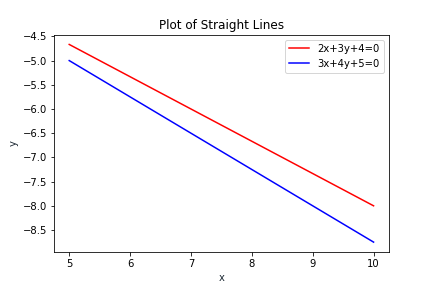
\includegraphics[width=\columnwidth]{st1.png}
	\caption{Plot of Straight lines when $h=\frac{17}{2}$}
	\label{myfig}
\end{figure}\\

Similarly, Sub $h=\frac{171}{20}}$ in equation \eqref{eq:question} we get,
\begin{align}
20x^2+57xy+40y^2+\frac{220}{3}x+\frac{310}{3}y+\frac{200}{3}=0 \label{eq:op2}
\end{align}
Rearranging equation \eqref{eq:op2},
\begin{multline}
\implies 20x^2+32xy+40x+
25xy+40y^2+50y+\\
\frac{100}{3}x+\frac{160}{3}y+\frac{200}{3}=0\\
\implies 4x(5x+8y+10)+5y(5x+8y+10)\\
+\frac{20}{3}(5x+8y+10) = 0\\
\implies \boxed{(4x+5y+\frac{20}{3})(5x+8y+10) = 0} \label{eq:line2}
\end{multline}
\renewcommand{\thefigure}{\arabic{figure}}
\begin{figure}[h!]
	\centering
	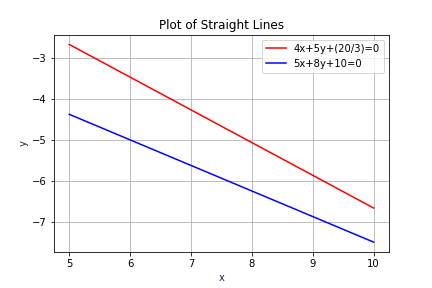
\includegraphics[width=\columnwidth]{st2.png}
	\caption{Plot of Straight lines when $h=\frac{171}{20}$}
	\label{myfig}
\end{figure}\\
\\\end{document}
